% !TEX root = ../Thesis.tex

\chapter{Theory}

\section{Electron Spin Resonance}
\subsection{Background Theory}

Electron spin resonance (EPR) functions by detecting the energy difference between the spin states of an electron.
Normally degenerate, the presence of a magnetic field separates the two spin states parallel to it in energy - known as the Zeeman splitting \cite{Feher1959}.
The spin state parallel to the magnetic field has a lower energy whilst the anti-parallel state has a higher energy.
These are described as the up, $\ket{\uparrow}$, and down, $\ket{\downarrow}$, spin states.
For an electron in free space the energy difference is given by:

\begin{equation}
\Delta E = g_e\mu_bB,
\label{eq:enSplit}
\end{equation}

where $g_e$ is the free electron g-factor, $\mu_b$ is the Bohr magneton and $B$ is the magnetic field strength. 
This results in an energy splitting as seen in figure \ref{fig:elecSplit}. 

\begin{figure}
\centering
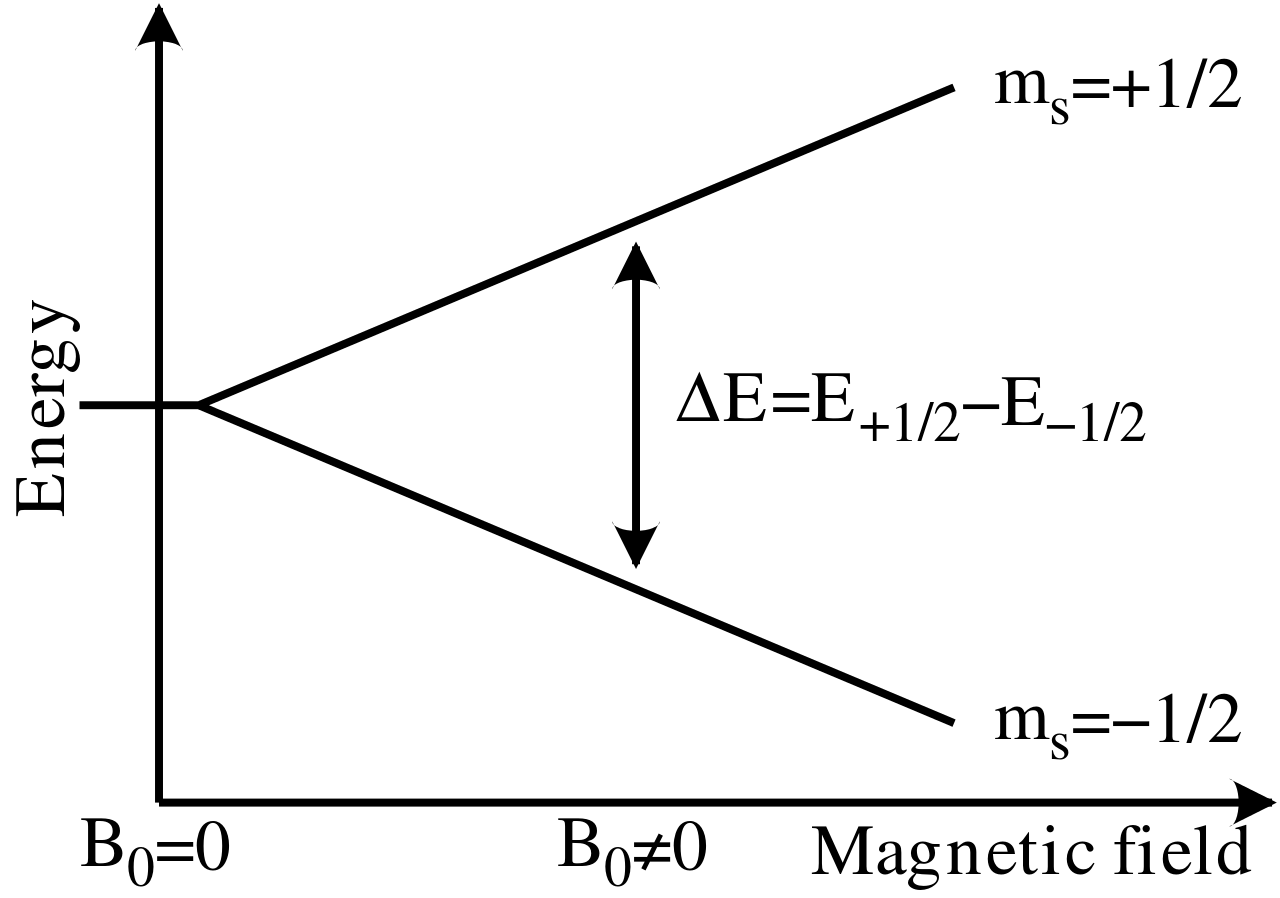
\includegraphics[width = 0.5\columnwidth]{Figures/EPR_splitting.png}
\caption[Free electron level splitting]{Spin state energy splitting for a free electron in a magnetic field.}
\label{fig:elecSplit}
\end{figure}

In practice this energy splitting can be detected using continuous wave EPR. Transitions between the spin states will be driven by incident electromagnetic radiation of photon energy equal to the energy gap (i.e $h\nu = g_e\mu_bB$). 
The presence of an EPR transition in a sample can be detected either by applying a constant magnetic field and sweeping EM frequency incident on that sample or vice versa.
In practice, it is the latter that is used for experimental simplicity.
Measuring reflection of radiation from the sample whilst sweeping magnetic field will reveal a drop in reflection at the transition field - when photons are absorbed by spins moving from the lower to higher energy state.

\subsection{Pulsed Electron Spin Resonance and Qubits}
The description above details continuous wave (CW) ESR, a technique that has proven invaluable for studying the electronic structure of materials.
Another ESR technique has proven more popular for the manipulation of spins for use as qubits: pulsed ESR.
This uses short bursts of microwave radiation, on resonance with the spin transition, to control spin states and allows the spin to function as a qubit.
This control is achieved by placing the spins at the centre of a cavity which produces a magnetic field when a pulse is applied.
This magnetic field causes precession which can be used to rotate the spins. 
Pulses are described in terms of a rotation angle, with a $\pi$ pulse taking  the ensemble of spins from the down to up state or vice versa. 
A $\pi/2$ pulse takes the spins into the plane normal to the magnetic field, termed the $x-y$ plane. 
This causes the spins to precess in the static magnetic field at the Lamor frequency given by:
\begin{equation}
\label{eq:larmor}
\omega = \frac{eg}{2m}B_0
\end{equation}

\subsubsection{Hahn Echo and Detection}

In pulsed ESR the spins are detected via the electromagnetic radiation they emit when precessing in a magnetic field. 
This radiation is of the same frequency as the resonant control radiation (easily shown using equations \ref{eq:enSplit} and \ref{eq:larmor}).
This emitted radiation can be demodulated with the control radiation giving a DC signal.
In a perfectly homogeneous magnetic field all spins would precess at the same rate giving a constant DC signal. In reality however, all spins will precess at slightly different rates due to small, static differences in the magnetic field each experiences.
So, following a $\pi/2$ pulse, the signal from the spins will rapidly decay as the ensemble of spins lose phase coherence. 
A technique, known as a spin or Hahn echo, to reverse this loss of phase was developed by Erwin Hahn in 1950 \cite{hahn1950}. 
This follows a $\pi/2$ pulse with a $\pi$ pulse after a set time interval, $\tau$. 
\textit{Static} magnetic field differences now act to reverse the loss of phase coherence. 
This results in a brief re-phasing of the spins following another interval $\tau$, detected as a rise and fall of a DC signal or an `Echo'.
A cartoon of this sequence is shown in figure \ref{fig:HahnEcho}. 

\begin{figure}
\centering
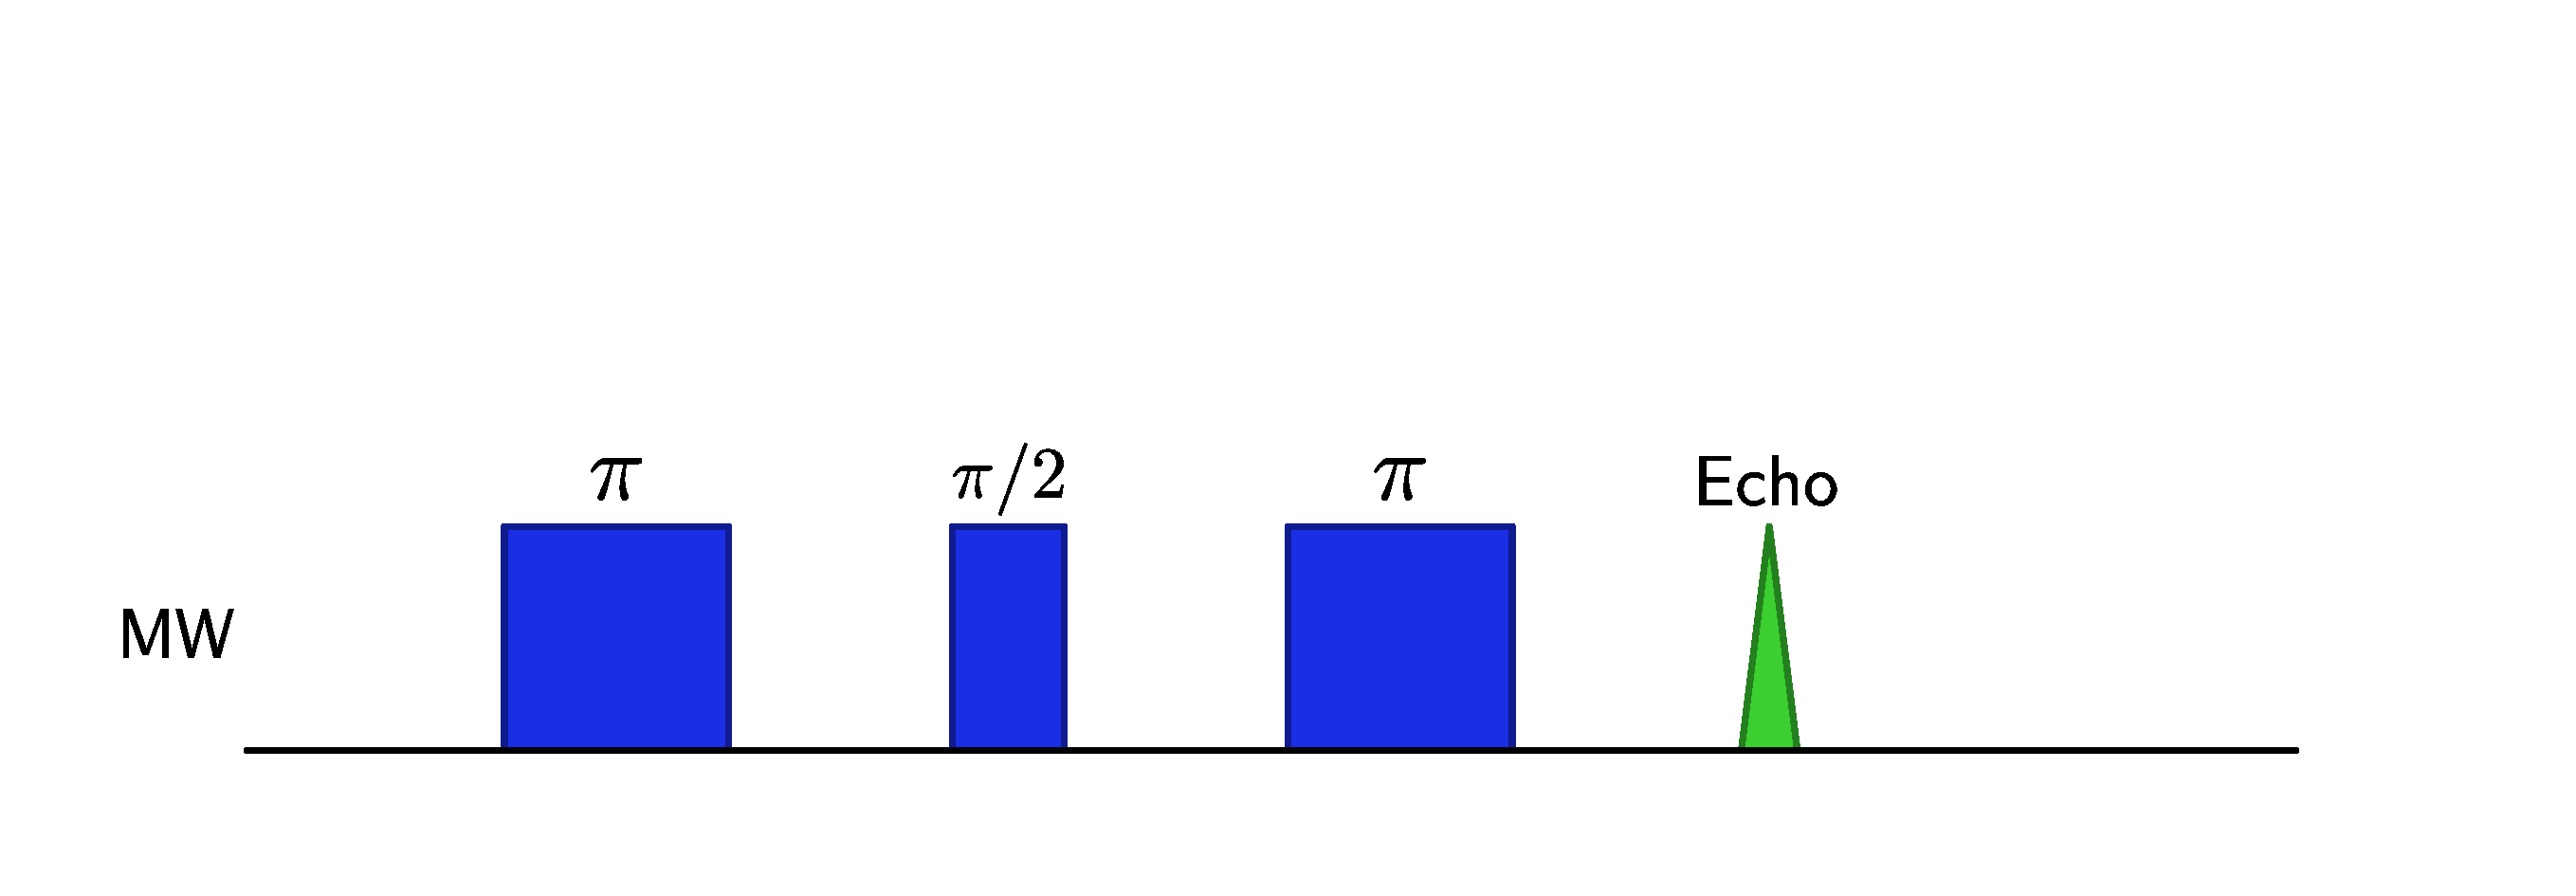
\includegraphics[width = \columnwidth]{Figures/hahnEcho.pdf}
\caption[Hahn echo sequence]{Cartoon showing a Hahn echo pulse sequence. A $\frac{\pi}{2}$ pulse causes the spins to precess in the $x-y$ plane. Loss of phase coherence is reversed via a $\pi$ pulse following time interval $\tau$ and a signal is detected following another interval of $\tau$.}
\label{fig:HahnEcho}
\end{figure}


\subsubsection{The Bloch Sphere}

The control pulses produce a magnetic field that rotates at the same rate as the spins, meaning a fixed coordinate system can be defined.
The rotation axis of the control pulses can be changed by varying their phase, for example a pulse of 0 phase is defined as a rotation about the $x$ axis whilst a pulse of $\pi/2$ phase is a rotation about the $y$.
This allows control of the direction of the spin vector in 3-D space, with the $z$-axis defined by the static magnetic field.  
A qubit, the basic unit of a quantum computer, can be described as a point within a unit sphere, known as a Bloch sphere and shown in figure \ref{fig:blochSphere} \cite{Nielsen:2011:QCQ:1972505}.
Clearly then, a single spin is an archetypal qubit: its eigenstates of $\ket{\uparrow}$ and $\ket{\downarrow}$ form the poles of the Bloch sphere. 
Microwave pulses of defined duration and phase enable the creation of an arbitrary linear superposition that allows the initialisation of any state on the surface of the Bloch sphere.
In the case of ESR, however, a huge number ($10^{10}$) of spins is being addressed. 
Although this means that they do not represent a true qubit, measurements of ensemble properties give great insight into the behaviour of single spins.
It is therefore prudent to establish the anticipated behaviour of the various potential spin qubit candidates using the comparatively simple experimental techniques of ESR before making the challenging step to single spin control and measurement. 

\begin{figure}
\centering
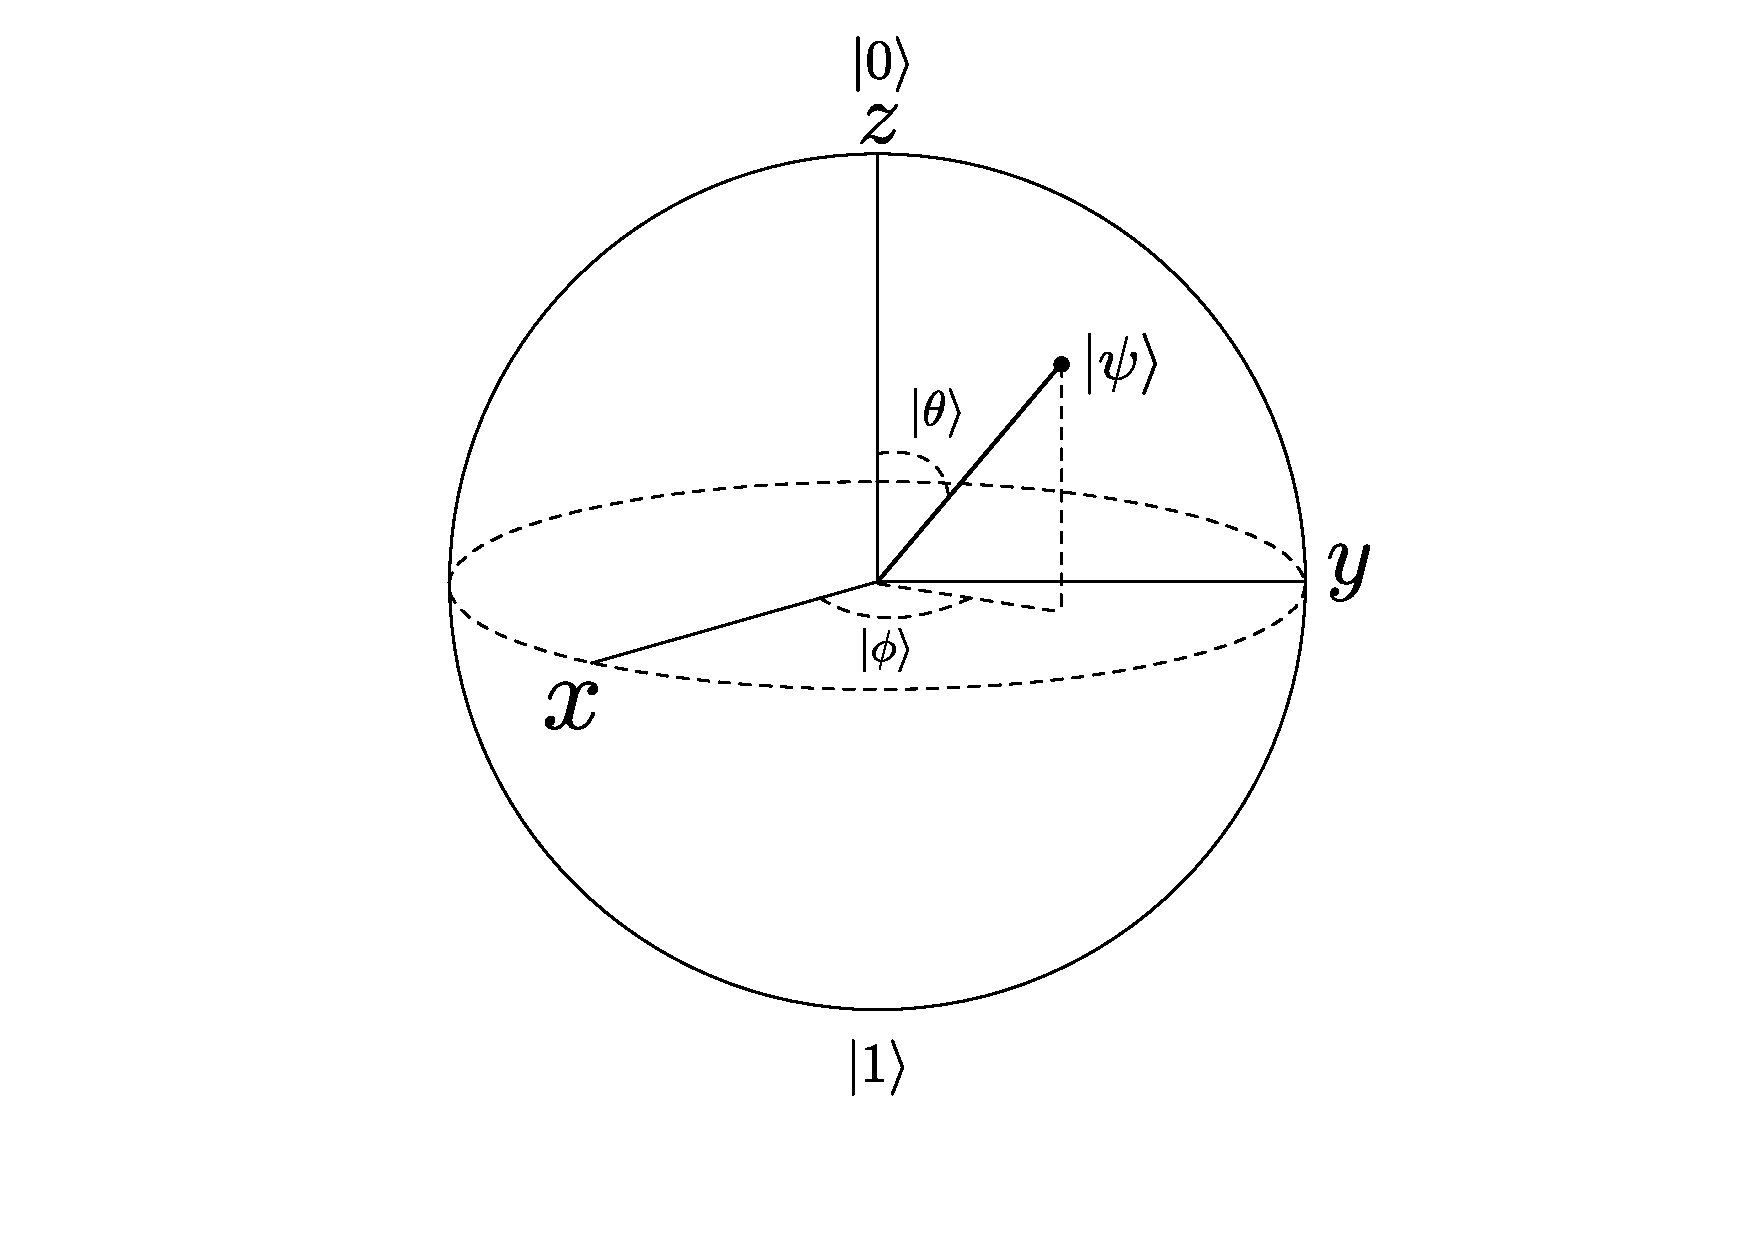
\includegraphics[width = 0.8\columnwidth]{Figures/blochSphere.pdf}
\caption[Bloch Sphere]{Diagram of the Bloch sphere - the most common representation of a qubit. The poles of the sphere at $\pm z$ represent the $\ket{0}$ and $\ket{1}$ or $\ket{\uparrow}$ and $\ket{\downarrow}$ states. Any point on the surface of the sphere represents some linear superposition of these two states. The state vector of any point is given by: $\ket{\psi} = \cos{\theta/2}\ket{0} + e^{i\phi}\sin{\theta/2}\ket{1}$}
\label{fig:blochSphere}
\end{figure}

\section{Donor States in Silicon}

\subsection{The Hyperfine interaction}

Discussion so far has focussed on single electrons in a magnetic field.
The spins discussed in this thesis will be those of the electrons and nuclei of donors in silicon.
For these spin states the situation is a little more complicated than the case of a free electron.
For all the donors discussed here, there is a nuclear as well as electron spin.
This introduces first an additional term in the Hamiltonian of the system due to the nuclear spin's Zeeman interaction with the magnetic field.
On top of the separate Zeeman interactions there is an additional interaction between the nucleus and the electron, known as the hyperfine interaction.
This term is due to the magnetic field of the electron interacting with the magnetic dipole moment of the nucleus.
This strength of this interaction is proportional to the overlap between the electron and nuclear wavefunctions.
The result of this is that it is preferential energetically for the electron and nuclear spins to be anti-aligned.
A further term in the Hamiltonian is due to the nuclear quadrupole but this effect is small enough to be neglected in this treatment.
These effects leave a Hamiltonian of the following form:
 
\begin{equation}
\label{eq:spinHam}
\hat{H} = \mu_bg_eB_0\hat{S_z} + \mu_ng_nB_0\hat{I_z} + A \hat{S}\cdot\hat{I},
\end{equation}

where $\mu_b \text{\&} \mu_n$ are the Bohr and nuclear magnetons, $g_e \text{\&} g_n$ are the electron and nuclear g-factors, $\hat{S} \text{\&} \hat{I}$ are the electron and nuclear spin operators, and $A$ is the hyperfine interaction term.
In general they hyperfine term is a tensor but due to the isotropic nature of silicon can be represented as a scalar here.

\subsection{Spin Transitions}

The electron spin is restricted to be $\pm \frac{1}{2}$, but the nuclear spin can take a much greater range of values. 
The nuclear spin of a phosphorus donor in silicon is $\pm \frac{1}{2}$, by contrast for a bismuth spin it can take the values $-\frac{9}{2}, -\frac{7}{2},...\frac{7}{2},\frac{9}{2}$. 
In the simple case of phosphorus this results in the four energy levels seen in figure \ref{fig:phosLevels}.

\begin{figure}[t!]
\centering
\begin{subfigure}[t]{0.7\columnwidth}
\centering
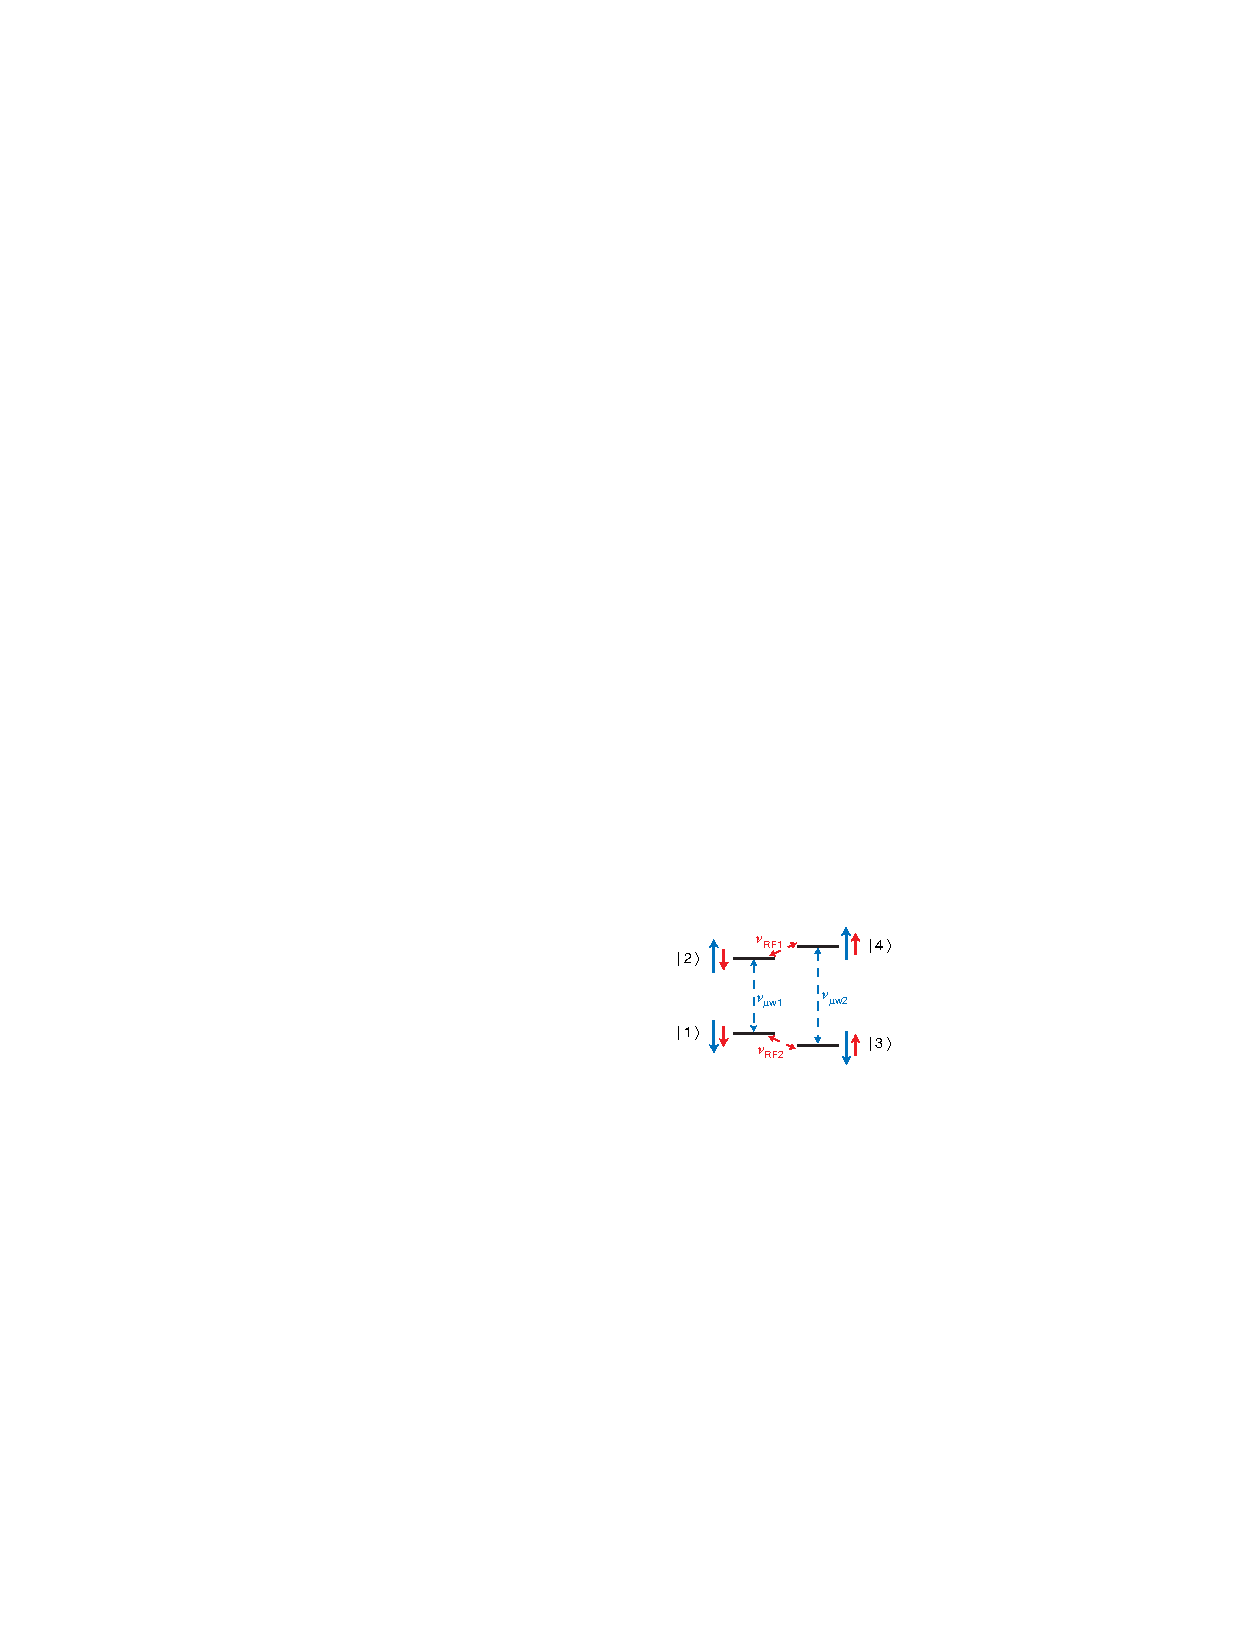
\includegraphics[width = \columnwidth]{Figures/phosphorus.pdf}{(a)}
\end{subfigure}
~
\begin{subfigure}[t]{0.7\columnwidth}
\centering
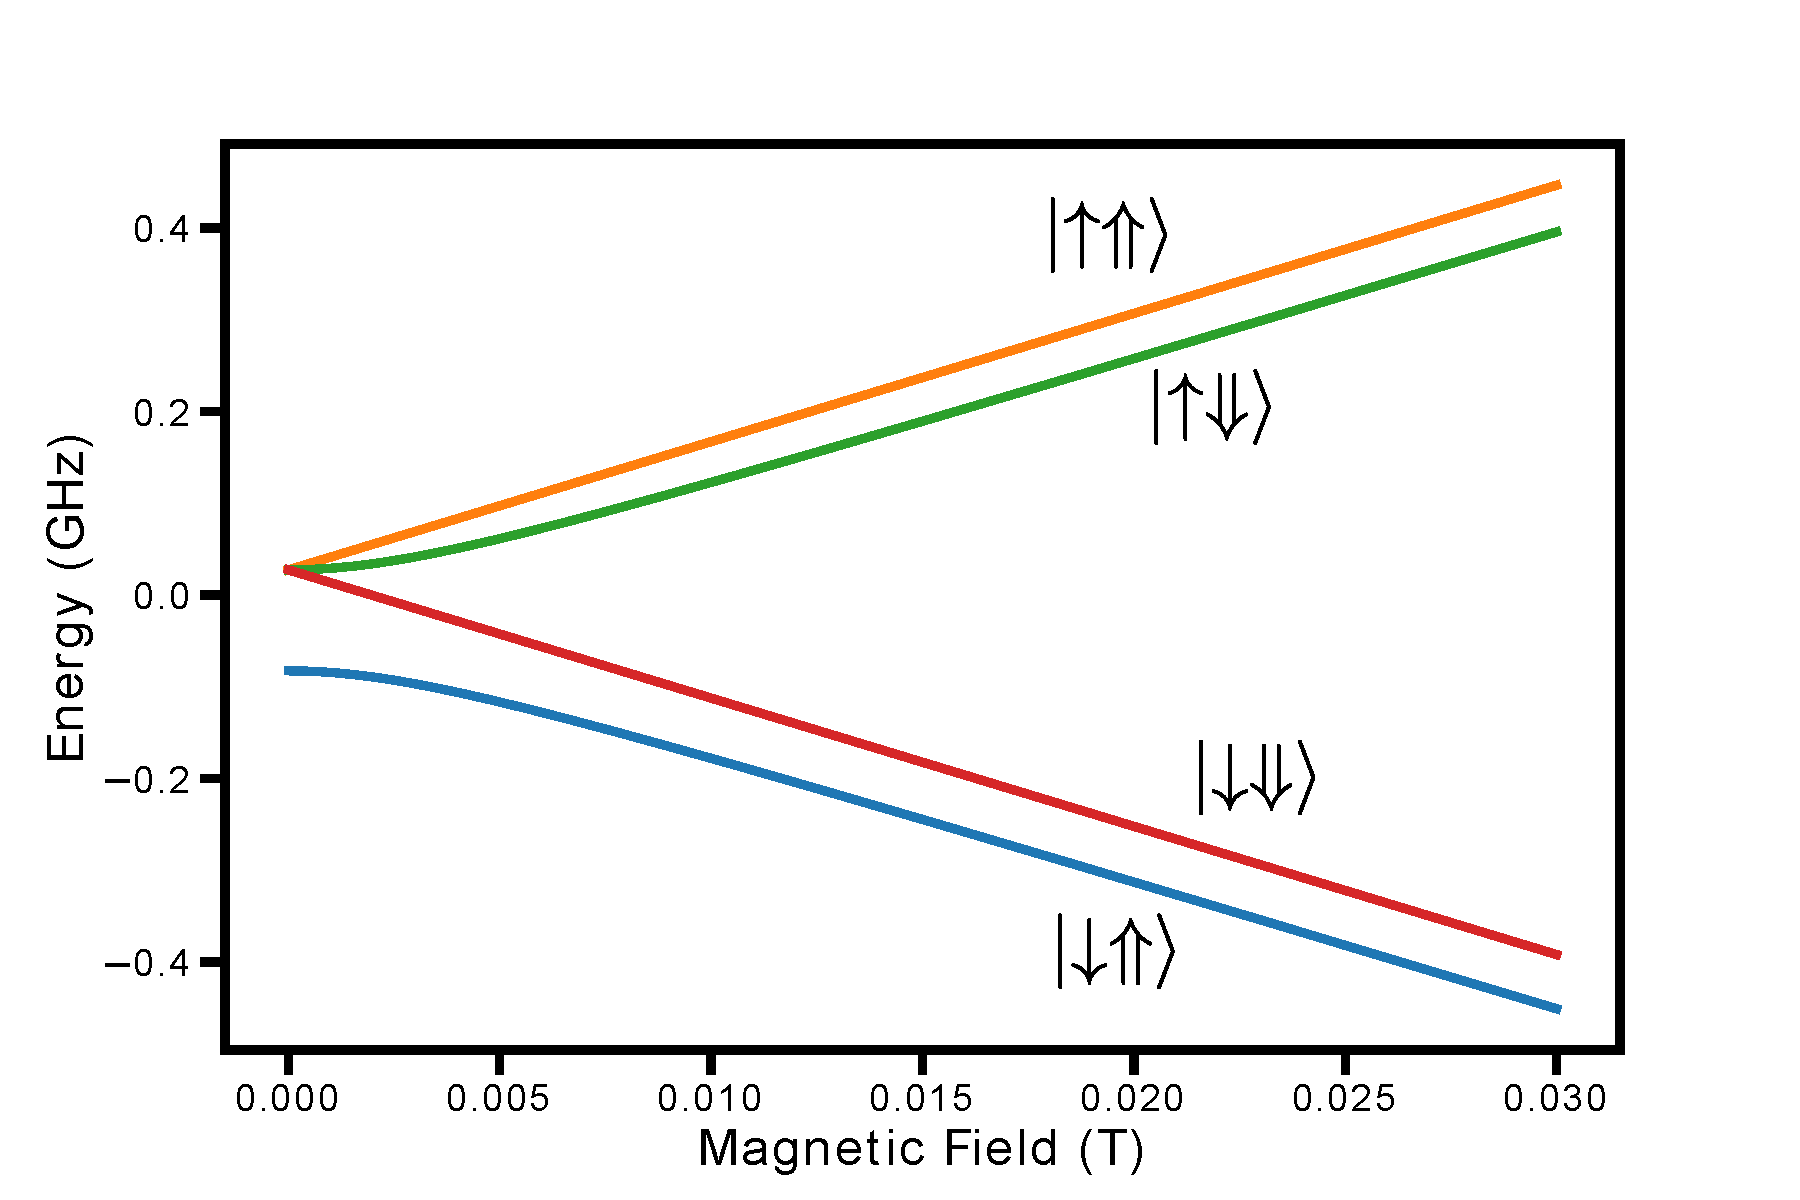
\includegraphics[width = \columnwidth]{Figures/fields.pdf}{(b)}
\end{subfigure}
\caption[Phosphorus energy levels and transitions]{Cartoon in a shows the relative energy levels for the different spin states of phosphorus in a high field environment. Note that in this case the electron Zeeman interaction dominates the hyperfine term which dominates the nuclear Zeeman term. b shows the simulated energies for each of the four possible states of the system.}
\label{fig:phosLevels}
\end{figure}

For the more complex case of bismuth, instead of 4 possible energy levels there are 20. 
Not all transitions are possible - spins are changed by the absorption or emission of a photon, only allowing transitions where the total spin changes by $\pm1$.
This means that only nuclear or electron spin can be flipped at once, not both. 
It should be clear that the transitions that involve an electron spin flip ( e.g. $\ket{\uparrow \Uparrow} \longrightarrow \ket{\downarrow \Uparrow}$) are significantly higher in energy than those involving a nuclear spin flip (e.g. $\ket{\uparrow \Uparrow} \longrightarrow \ket{\uparrow \Downarrow}$). 
At typical experimental magnetic fields ($\approx 0.3$ Tesla), the nuclear transitions are at frequencies of 10s of MHz, whilst the electron transitions are at $\approx 9.7$ GHz.
In addition to their different energies electron and nuclear transitions have different strengths or Rabi frequencies. 
The electron spin transition is much stronger and occurs on the order of nanoseconds at typical pulse powers, with the nuclear transition being on the order of microseconds.

\subsection{Relaxation Processes}
\label{sec:relProc}

For spins in silicon, three main relaxation or decoherence processes occur, causing the loss of information.
\\
\\
\textbf{Dephasing}
\\
\noindent\rule{\columnwidth}{1pt}
\begin{adjustwidth}{1.5cm}{}
The first of these was briefly discussed above - dephasing - the time scale for the process is termed \textbf{$T_2^*$}
This is the process by which an ensemble of spins loses phase coherence due to each spin experiencing a different static magnetic field.
As was described above, this loss of information can be reversed by a Hahn echo sequence.
\end{adjustwidth}
\textbf{Relaxation} \newline
\noindent\rule{\columnwidth}{1pt}
\begin{adjustwidth}{1.5cm}{}
The second process is known as relaxation and its time scale is termed $T_1$. A spin ensemble at a given temperature and magnetic field will have a Boltzmann distributed population across the available spin states defined by the magnetic field axis (i.e. across the eigenstates of the $\hat{Z}$ operator).
The difference between higher and lower energy states is known as the polarisation of the ensemble.
If this polarisation is reversed by a $\pi$ pulse, then on a time scale $T_1$ it will relax back to thermal equilibrium.
As this process almost always involves interaction with the silicon crystal lattice it is also termed \textit{spin-lattice} relaxation.
This process is strongly correlated with temperature and exact mechanisms will be discussed in the literature review section.
\end{adjustwidth}
\textbf{Decoherence}
\\
\noindent\rule{\columnwidth}{1pt}
\begin{adjustwidth}{1.5cm}{}
The third process, decoherence, occurs on the time scale $T_2$. 
This is similar to the dephasing process described above but is irreversible. 
Irreversible phase differences are caused by by inhomogeneous and \textit{time dependent} magnetic fields. 
Additional phase acquired due to a time varying magnetic field will not be reversed by a Hahn echo sequence as the field will act differently on the spin in the second half of the sequence.
\end{adjustwidth}

\subsection{Summary}

The theory discussed above gives a background to the topics that will be discussed in detail during the literature review section of this report.
